\begin{figure*}[!tb]
	\centering
	\begin{subfigure}[t]{0.32\textwidth}
		\centering
		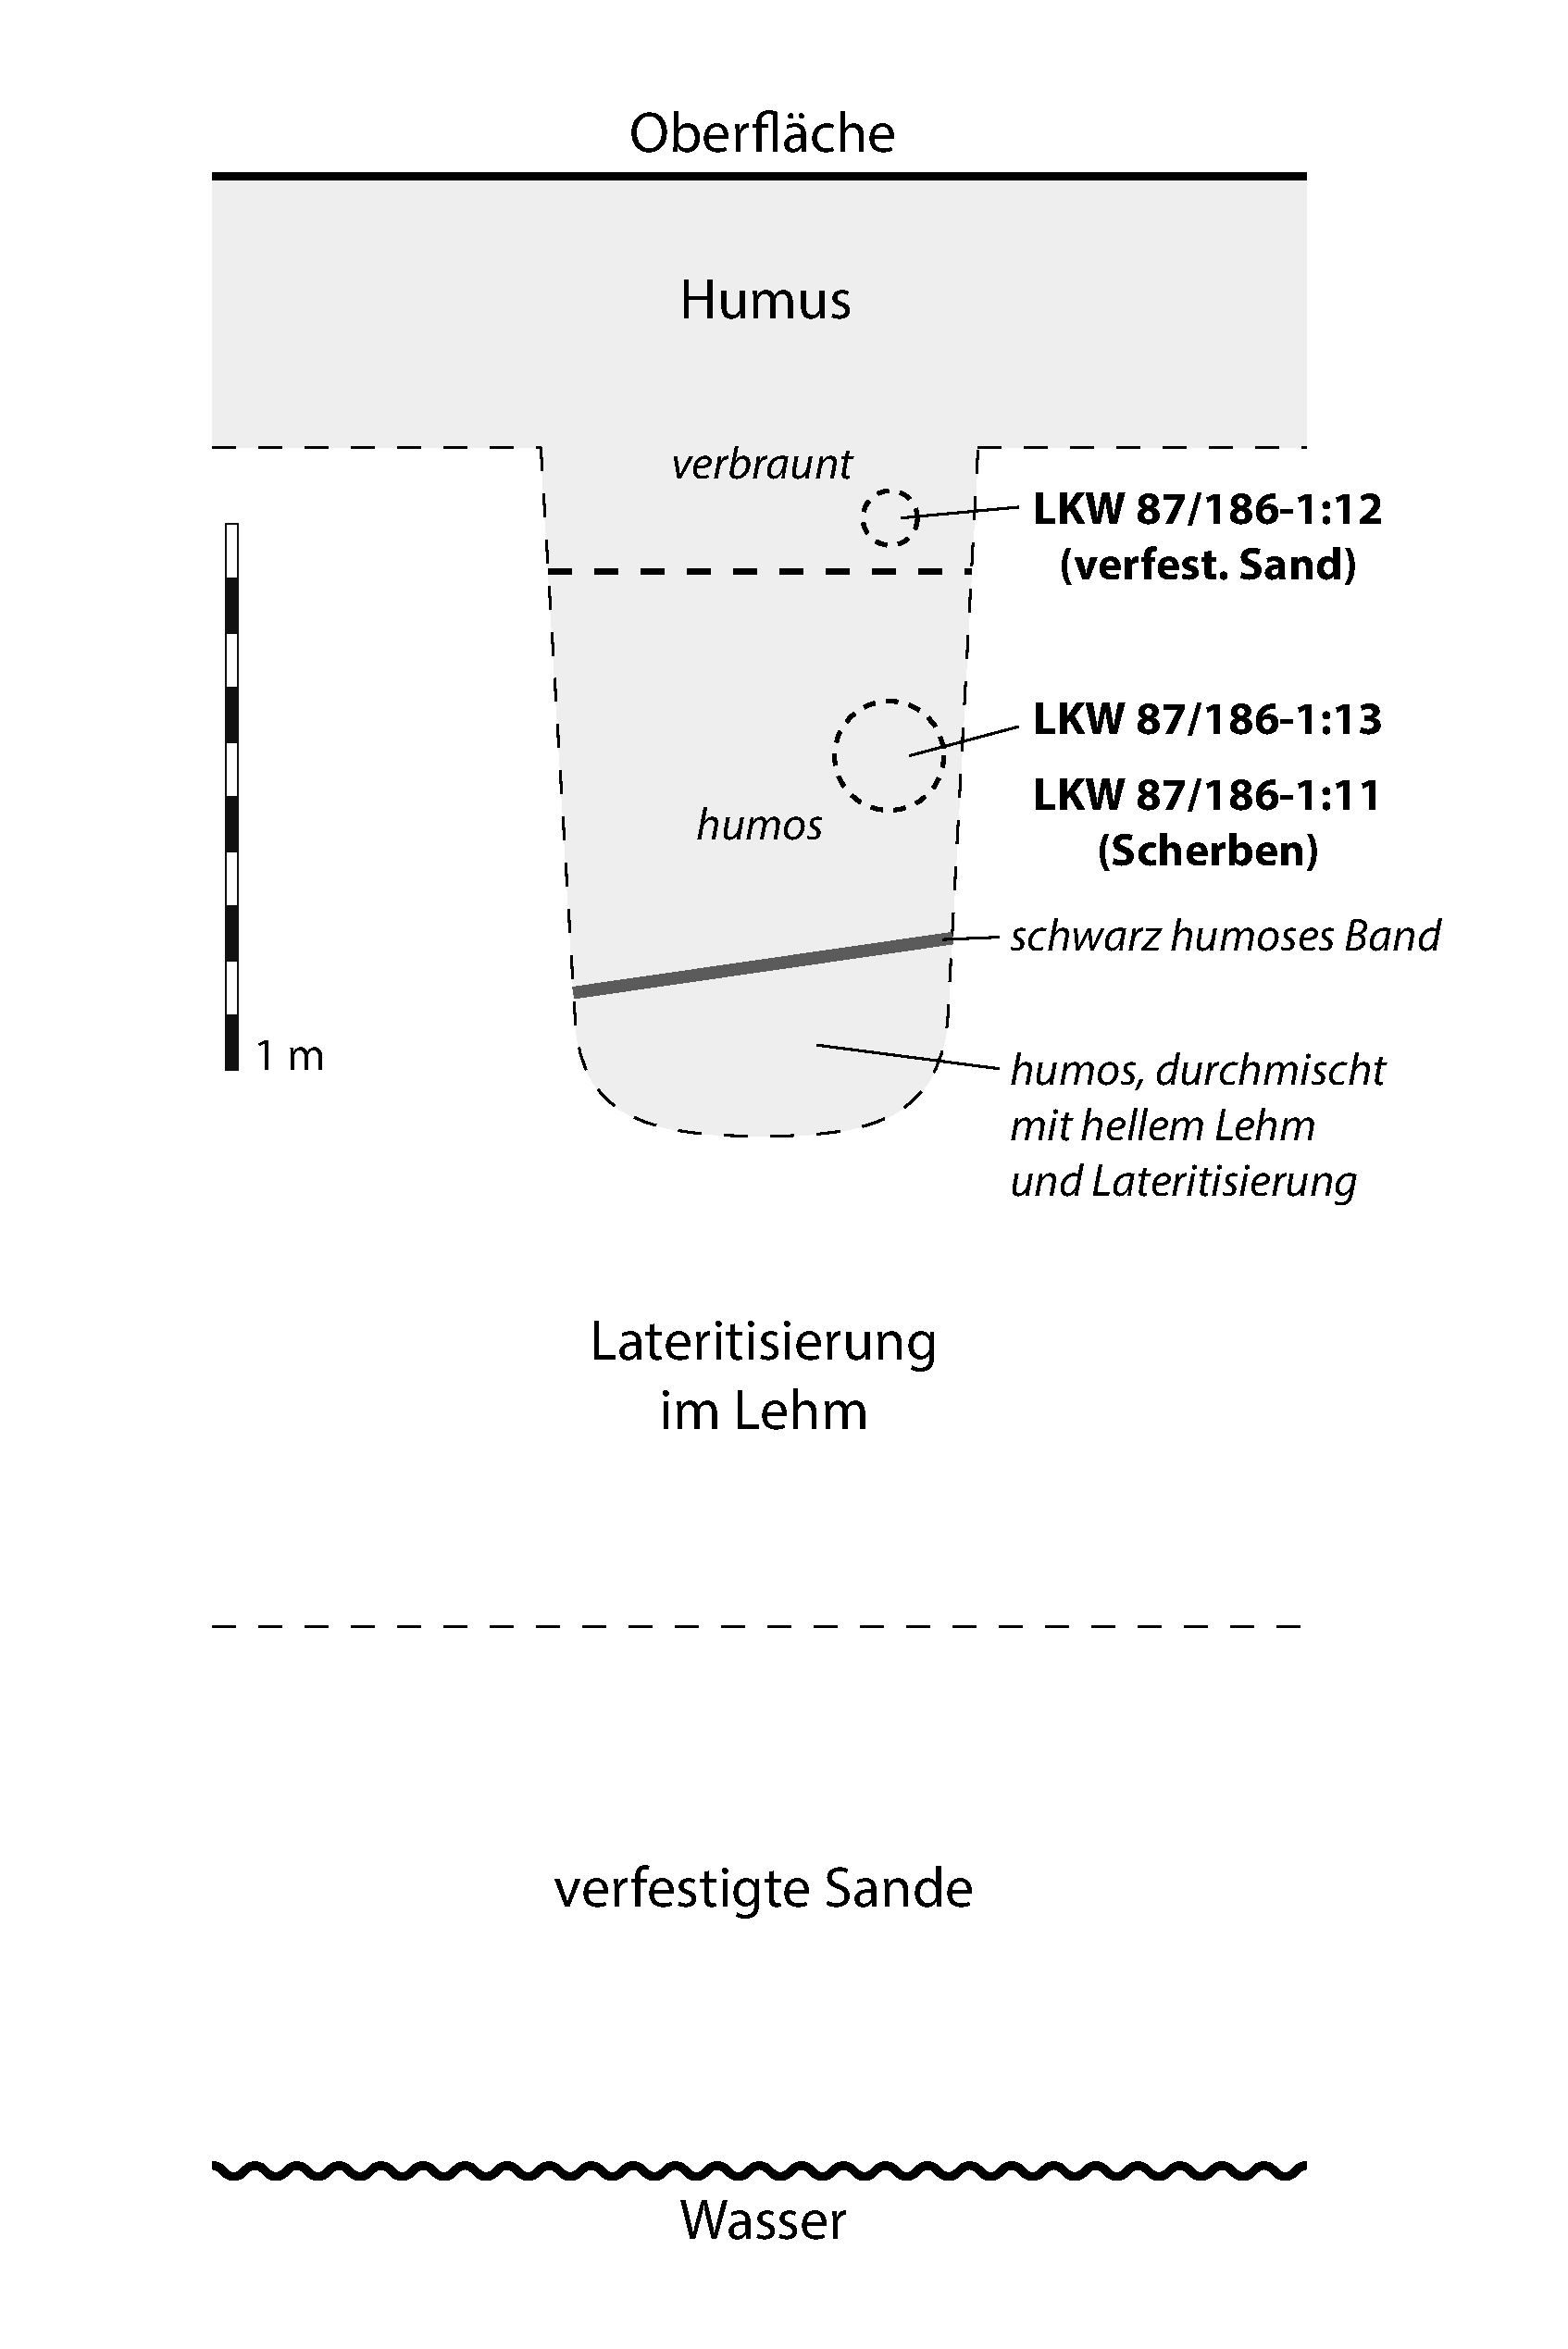
\includegraphics[width = \textwidth]{fig/LKW87-186.pdf}
		\caption{Vermessungsskizze.}
		\label{fig:LKW87_186_Skizze}
	\end{subfigure}\hfill
	\begin{subfigure}[t]{0.32\textwidth}
		\centering
		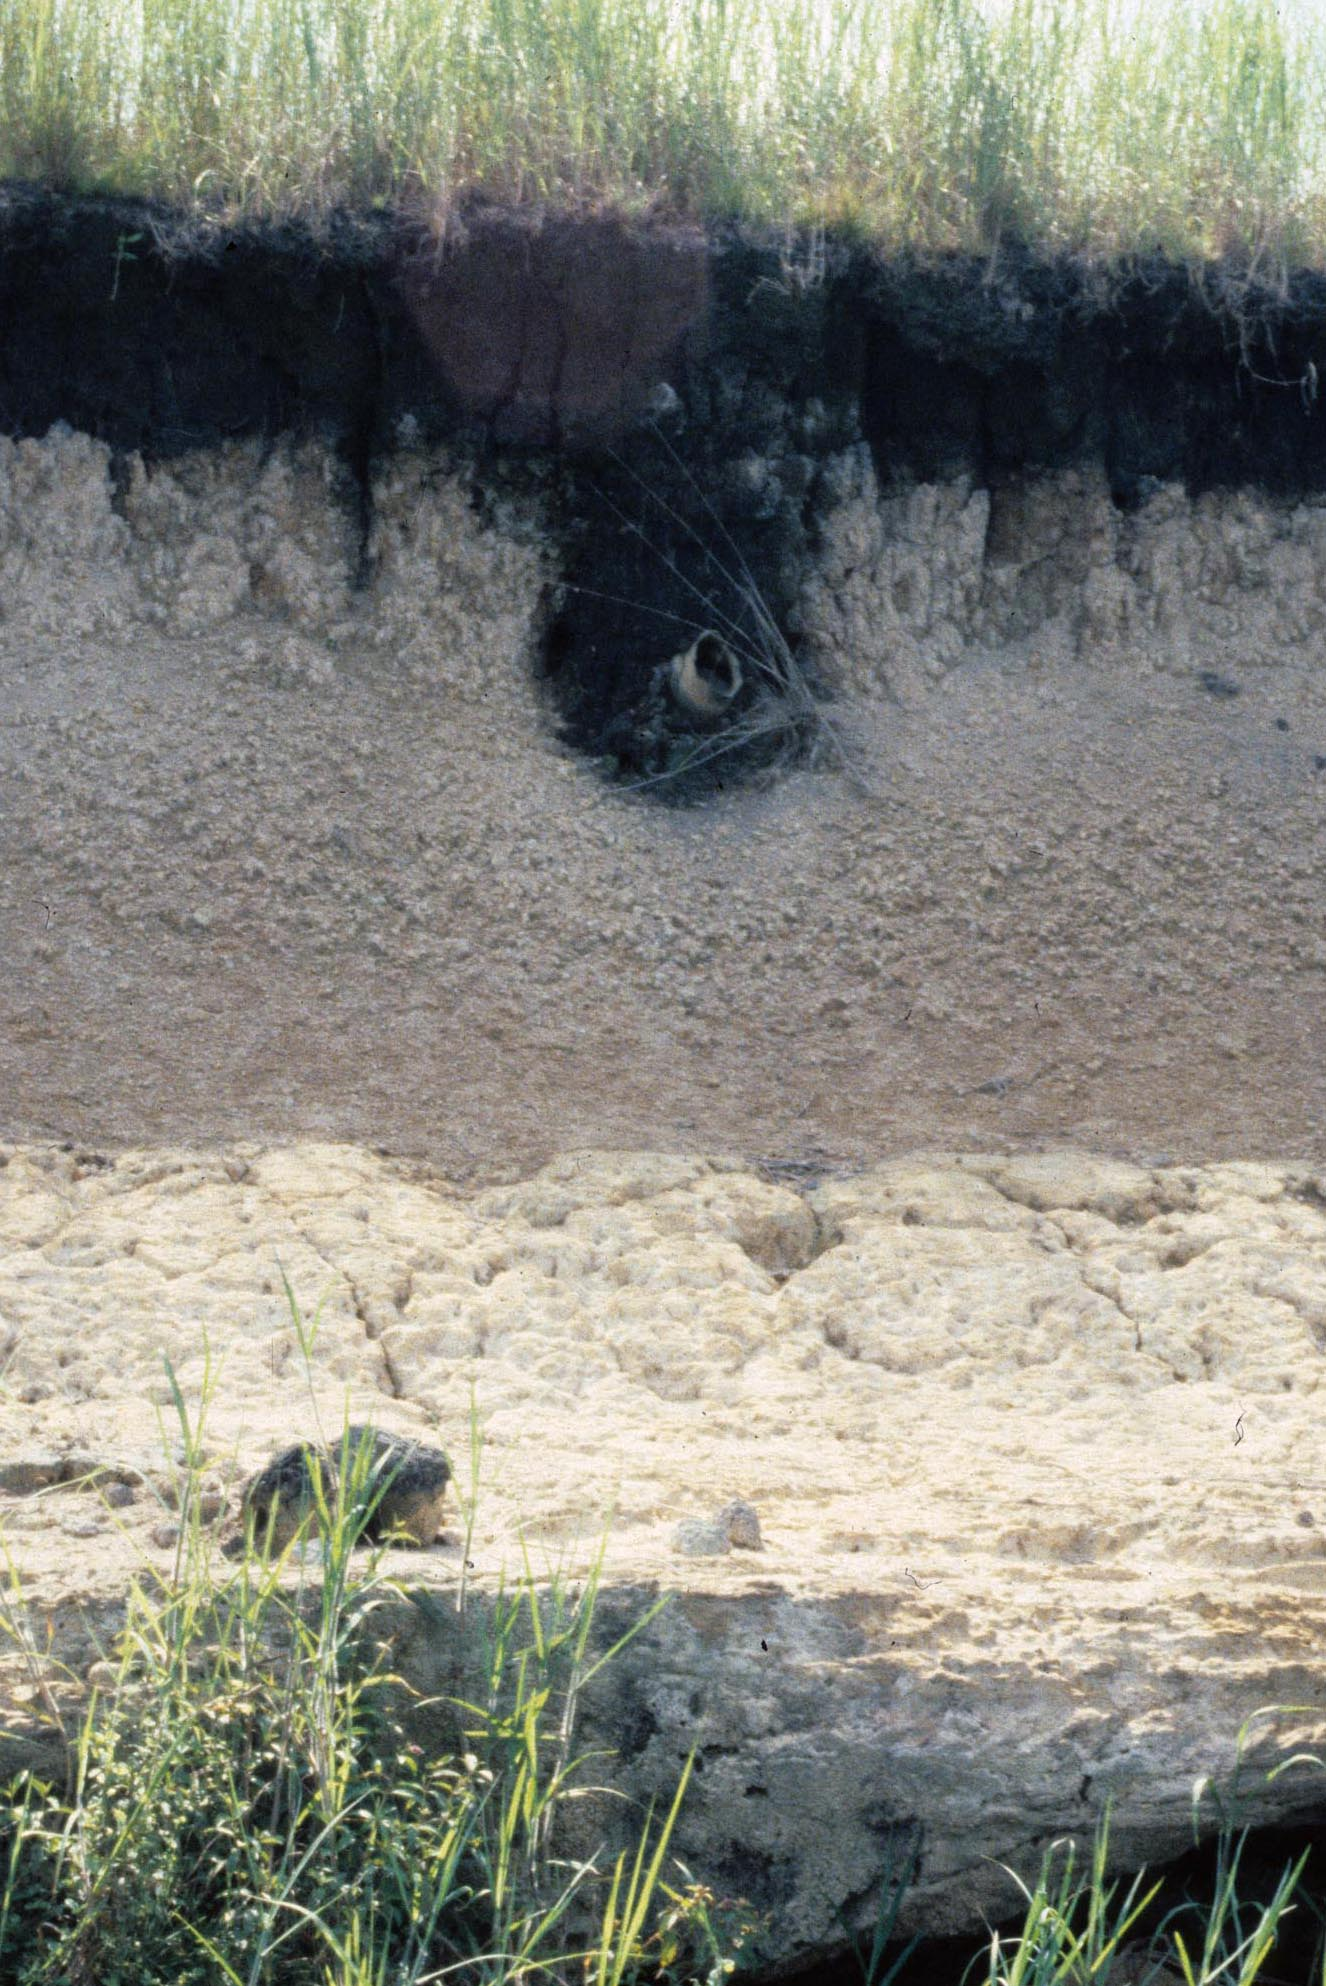
\includegraphics[width = \textwidth]{fig/LKW87-186_E87-047-3.jpg}
		\caption{Uferböschung.}
		\label{fig:LKW87_186_Foto}
	\end{subfigure}\hfill
	\begin{subfigure}[t]{0.32\textwidth}
		\centering
		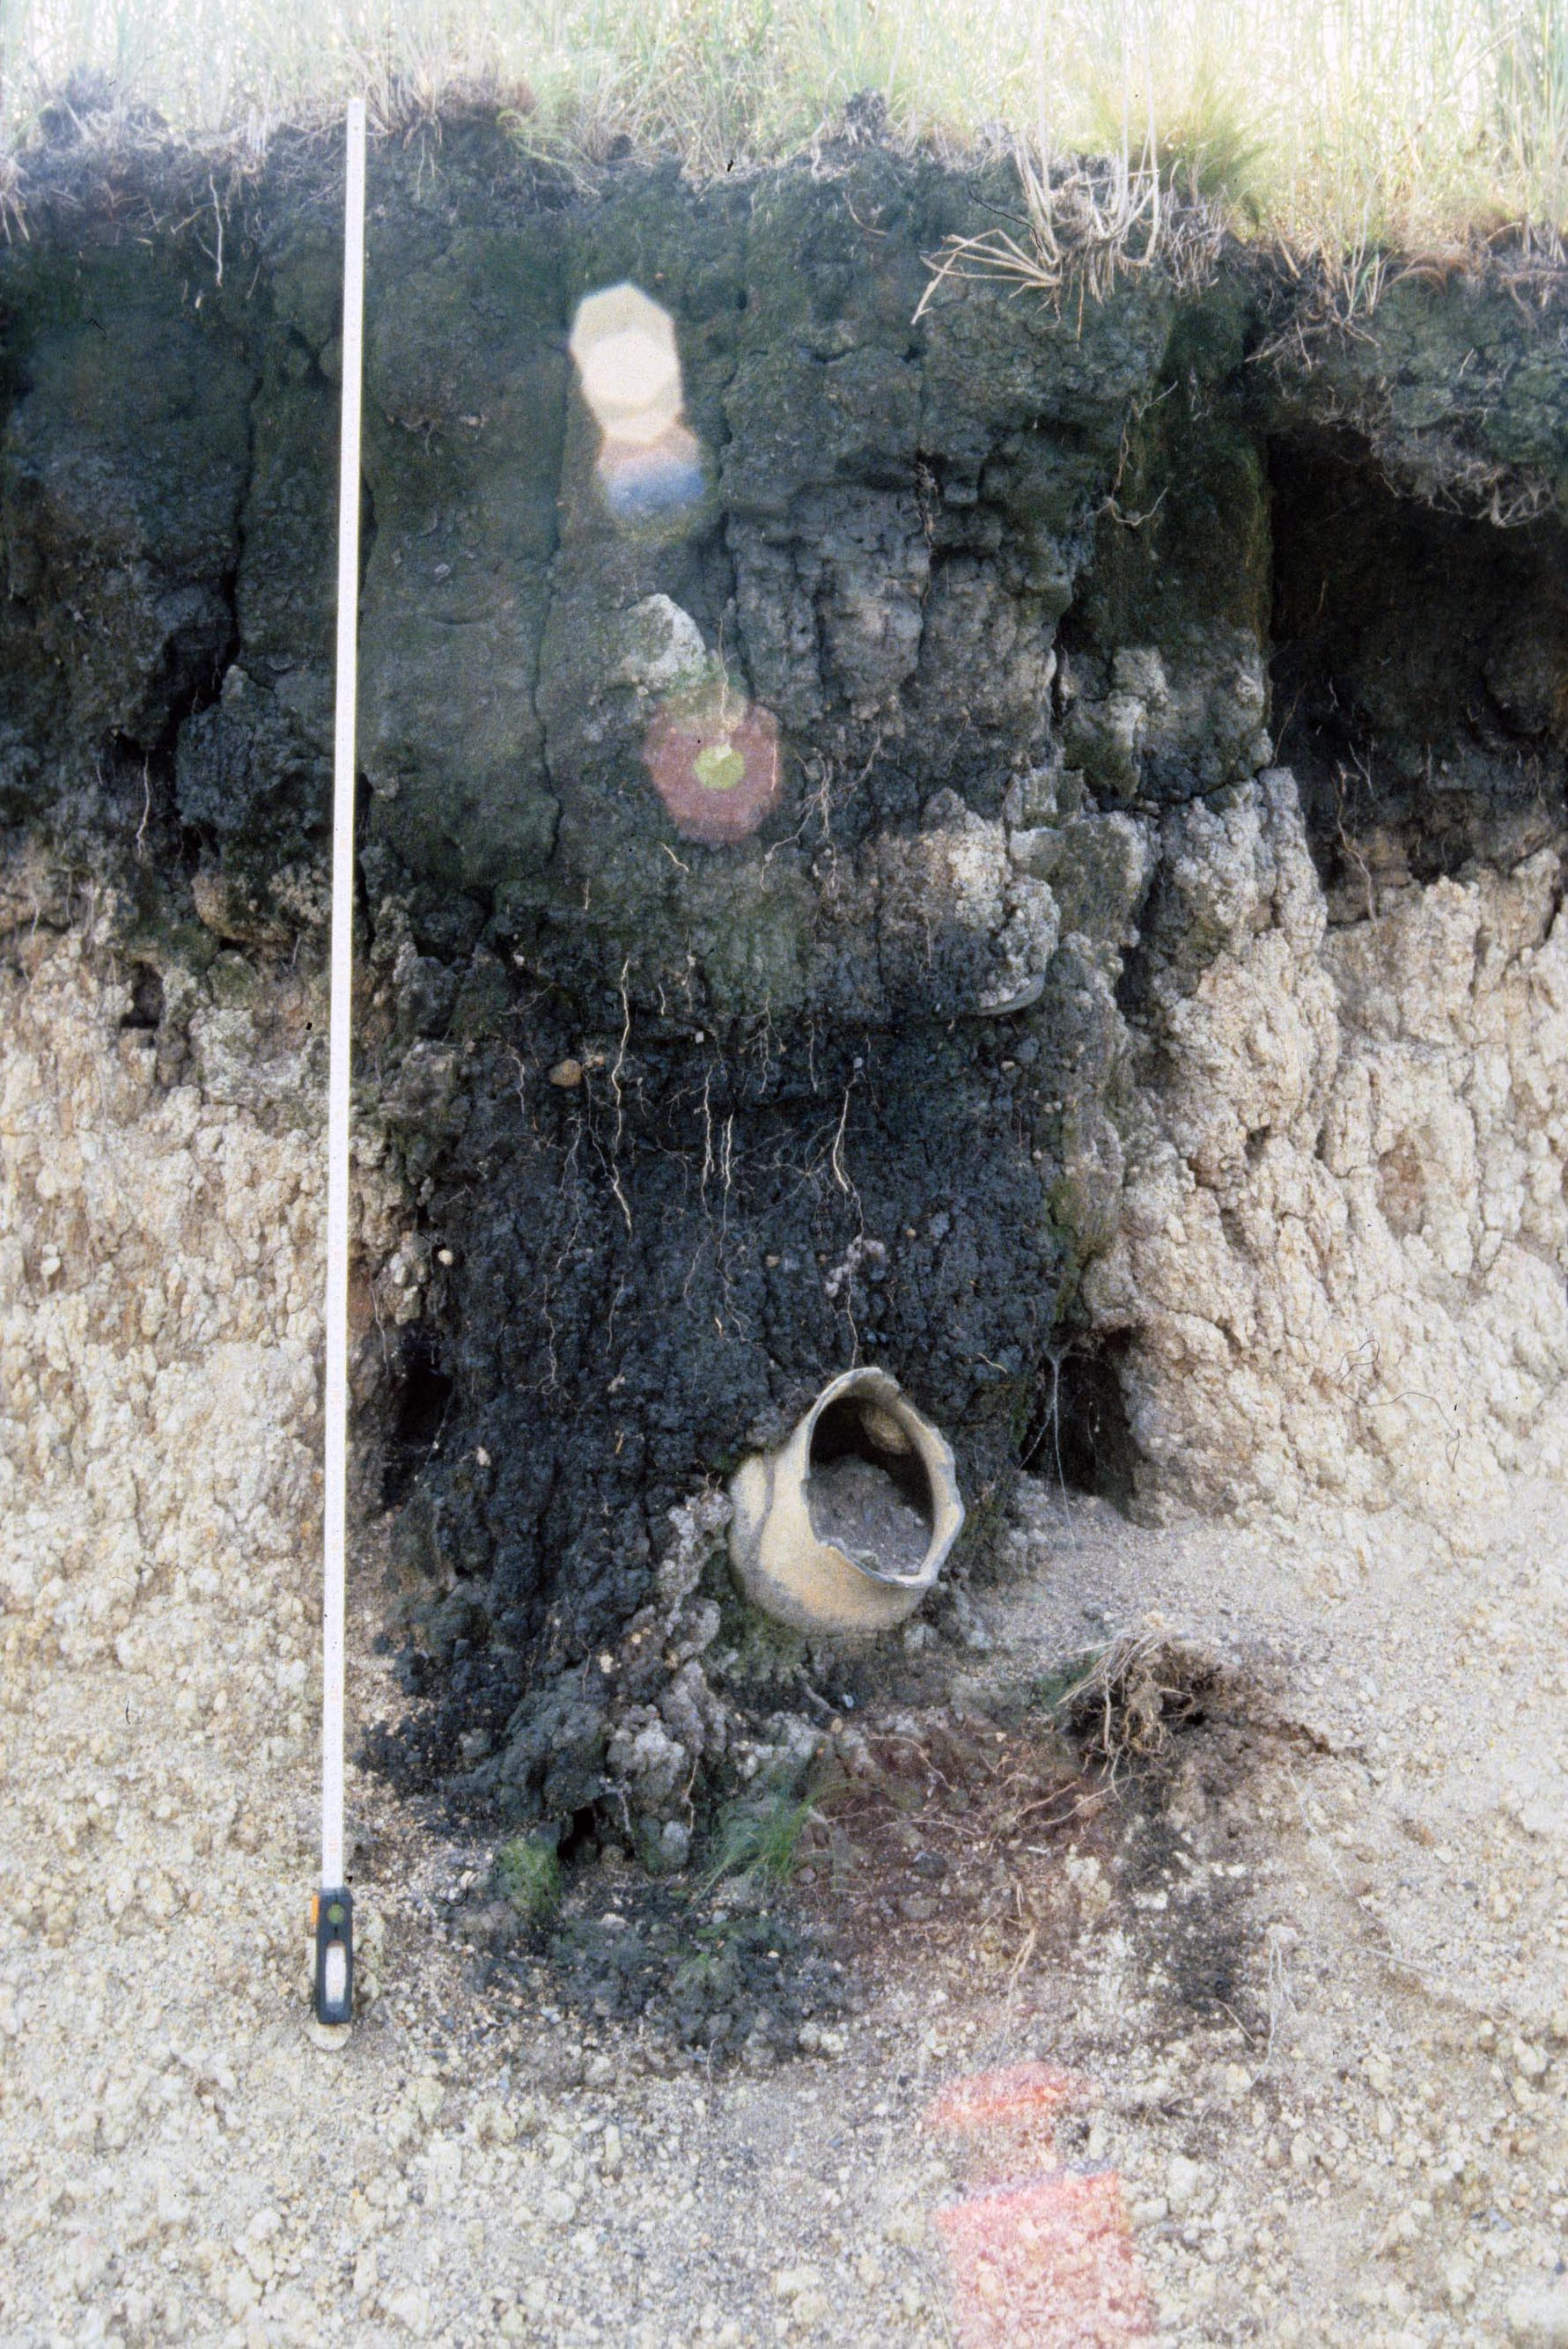
\includegraphics[width = \textwidth]{fig/LKW87-186_E87-047-4.jpg}
		\caption{Detail.}
		\label{fig:LKW87_186_FotoDetail}
	\end{subfigure}
	\caption{LKW 87/186: Übersicht und Detail des Befundes  (Fotos: M. K. H. Eggert, 1987).}
	\label{fig:LKW87_186}
\end{figure*}

\begin{table*}[!tb]
\centering
	{\footnotesize\begin{sftabular}{@{}lrrrr@{}}
\toprule
\textbf{Fundkategorie} &  \textbf{Anzahl} &    \textbf{\%} &  \textbf{Gewicht (kg)} &    \textbf{\%} \\
\midrule
      Keramik &      18 &  94,7 &          1,98 &  76,3 \\
        Stein &       1 &   5,3 &          0,61 &  23,7 \\
\bottomrule
\end{sftabular}
}
	\caption{LKW~87/186: Anteil verschiedener Fundmaterialien.}
	\label{tab:LKW87-186_Funde}
\end{table*}

\section*{\begin{tabular*}{\linewidth}{@{}l @{\extracolsep{\fill}} r@{}}
		Nr.~19 & LKW~87/186 \\
	\end{tabular*} 
}

\textsf{\textbf{Likwala-aux-Herbes Fluss-KM 186 (Likwala-aux-Herbes; Fpl.~291)}}

\vspace{1em}

\noindent\begin{tabular}{@{}rl@{}}
	\textbf{Feldarbeit:} & \begin{tabular}[t]{@{}l@{}}\textbf{02.09.1987 (F. Nikulka/}\\ \textbf{H. Holsten)}\end{tabular} \\ 
	\textbf{Abb.:} & \textbf{\ref{fig:LKW87_186}} \\ 
	\textbf{Tab.:} & \textbf{\ref{tab:LKW87-186_Funde}}\\
	\textbf{Taf.:} & \textbf{76.1--11} \\ 
	\textbf{Lit.:} & \textbf{\textsc{Eggert} 1993} \\ 
\end{tabular} 

\paragraph{Grabung und Befunde}\hspace{-.5em}|\hspace{.5em}%
Bei Flusskilometer 186 wurde in der westlichen, aus Tonen und alluvialen Sedimenten bestehenden Uferböschung des \mbox{Likwala}-\mbox{aux}-\mbox{Herbes} eine teilweise freierodierte Grube beobachtet (Abb.~\ref{fig:LKW87_186_Foto}). Aufgrund von Zeitmangel konnte keine systematische Untersuchung des Befundes durchgeführt werden. Es wurden lediglich Fotos sowie eine grobe Handskizze angefertigt und die sichtbare Keramik sowie eine Holzkohleprobe entnommen. Die halb im Uferprofil des \mbox{Likwala}-\mbox{aux}-\mbox{Herbes} angeschnittene Grube reichte bis 1,76\,m unter die heutige Oberfläche. Sie hatte einen Durchmesser von zirka 0,8\,m und wurde von einer etwa 0,5\,m mächtigen stark humosen Schicht überlagert.

\paragraph{Keramik\vspace{.5em}}\mbox{}\\
\begin{tabular}{@{}lrl@{}}
Bearbeitet:	& 1975\,g & (100\,\%) \\ 
\end{tabular} 

\vspace{1em}
\noindent Die aus der Grube stammende Keramik fällt aus dem bekannten Spektrum der im nordwestlichen Kongobecken beobacheteten Formen eindeutig heraus. Es handelt sich um hohe Formen mit leicht geschweifter Wandung, kurzen Hälsen und ausbiegenden Rändern vom Typ B2 (Taf.~76.3) sowie C1 (Taf.~76.1--2). Des Weiteren fand sich auch eine Schale mit geschweifter Wandung und einbiegendem Rand vom Typ H2 (Taf.~76.4). Da sich das Inventar nur aus wenigen GE zusammensetzt, sind belastbare Aussagen zur stilistischen Variabilität natürlich nicht möglich. Auch dass nur ein vollständiges Gefäß (Taf.~76.1) sowie vier hinreichend große Gefäßteile gefunden wurden (Taf.~76.2--3, 6, 11), erschwert die Ansprache des Komplexes.\footnote{Die übrigen Scherben waren durchweg kleiner als 70\,$\times$\,70\,mm.} Die Verzierungen finden sich vor allem auf den Rändern, Gefäßschultern und \mbox{-bäuchen}. Es handelt sich häufig um technisch \textit{einfach} oder \textit{grob} ausgeführte Verzierungselemente aus Rillenbündeln (Tab.~\ref{tab:Verzierungselemente}: 02.1), rillengefüllten Bändern (Tab.~\ref{tab:Verzierungselemente}: 02.4) und Kreuz-Mustern (Tab.~\ref{tab:Verzierungselemente}: 01.11). Die Stücke weisen durchweg keine nichtplastischen Partikel im Scherben auf und lassen sich dem \textit{Fabric}~1 zuordnen. Sie unterscheiden sich damit kaum von grundsätzlich zeitgleichen GE des Pikunda-Munda-Stils (Kap.~\ref{sec:PKM-Gr}).

Schwache stilistische Parallelen ergeben sich zu einem Gefäß aus Gbadolite am Oberlauf des \mbox{Ubangi} \parencite[277; 278 Abb. 7]{Eggert.1984}, den Funden von der Île des Mimosas \parencite[279 Abb. 8]{Eggert.1984} und der Ngovo-Gruppe des Niederkongo (Kap.~\ref{sec:Niederkongo}). Nur zwei GE aus dem Befund weisen schwache Ähnlichkeiten zur Pikunda-Munda-Keramik auf: ein Fragment eines Gefäßes mit deutlich geschweifter Wandung und einem horizontalen Zierband auf Höhe des maximalen Bauchdurchmessers (Taf.~76.11) und ein kleines Fragment, das einen für die Schalen der Pikunda-Munda-Gruppe charakteristischen Bauchknick aufweist.\linebreak

Eine weitere Sonderrolle nimmt ein Fragment eines hohen Gefäßes mit langer Schulter und einem Bilobé-artigen Rand ein (Taf.~76.6). Dieses Stück ist das einzige im Inventar, dessen Scherben einen markanten Anteil gröberer nichtplastischer Partikel aufweist und nicht der gleichen Machart wie die übrigen Stücke entspricht.

\paragraph{Datierung}\hspace{-.5em}|\hspace{.5em}%
Eine Radiokohlenstoffdatierung (KI-2893) datiert den Befund in das 2.~Jh. v.~Chr.--3.~Jh. n.~Chr. Der Befund zählt damit mit zu den Ältesten absolut datierten im Arbeitsgebiet.

\paragraph{Interpretation}\hspace{-.5em}|\hspace{.5em}%
Mit der im Uferprofil des \mbox{Likwala}-\mbox{aux}-\mbox{Herbes} angeschnittenen Grube wurde ein Befund erfasst, dessen Fundinventar im Arbeitsgebiet gegenwärtig ohne Vergleich ist. Die zeitgleiche Keramik der Region, der Pikunda-Munda-Stil (Kap.~\ref{sec:PKM-Gr}), unterscheidet sich deutlich von der \mbox{Keramik} aus dieser Grube. Jedoch wurden auch nur wenige GE aus dem Befund geborgen und das Spektrum der Formen kann gegenwärtig kaum abgeschätzt werden. 

Die nächsten Vergleiche für die formalen Charakteristika der Keramik weisen auf das Gebiet des Pool Malebo (Kinshasa) sowie den Oberlauf des \mbox{Ubangi}. Die technischen Charakteristika lassen keine wirklichen Unterschiede zur zeitgleichen Keramik des Pikunda-Munda-Stils erkennen (Kap.~\ref{sec:Herstellung}). 

Über den Charakter des Befundes kann aufgrund der spärlichen Informationen keine Aussage gemacht werden. Die Tatsache, dass sich aber ein fast vollständiges Gefäß (Taf.~76.1) in der Grube fand, lässt einen Vergleich mit Keramikdeponierungen, wie sie im Inneren Kongobecken \parencite{Wotzka.1993} und auch in Munda (Kat.-Nr.~16--17) beobachtet werden können, nicht unwahrscheinlich erscheinen.